\documentclass[varwidth=false,border=7]{standalone}
\usepackage{tikz}
\usetikzlibrary{positioning,fit,calc}

% Define shape for "User"
\tikzstyle{user} = [rectangle, rounded corners, 
minimum width=3cm, 
minimum height=1cm,
text centered, 
draw=black, 
fill=green!30]

% Define shape for DNS
\tikzstyle{dns} = [rectangle, 
minimum width=3cm, 
minimum height=1cm,
text centered,
text width=3cm,
draw=black, 
fill=blue!30]

% Define shapes for clouds A and B
\tikzstyle{block_A} = [draw=black, thick,  minimum height=.5cm, align=center, fill=gray!50]  
\tikzstyle{block_B} = [draw=black, thick,  minimum height=.5cm, align=center, fill=white] 

% Define arrow styles
\tikzstyle{arrow} = [thick,->,>=stealth]
\tikzstyle{arrow_double} = [thick,<->,>=stealth]
\tikzstyle{arrow_dashed} = [dashed,->,>=stealth]
\tikzstyle{arrow_double_dashed} = [dashed,<->,>=stealth] 

\begin{document}

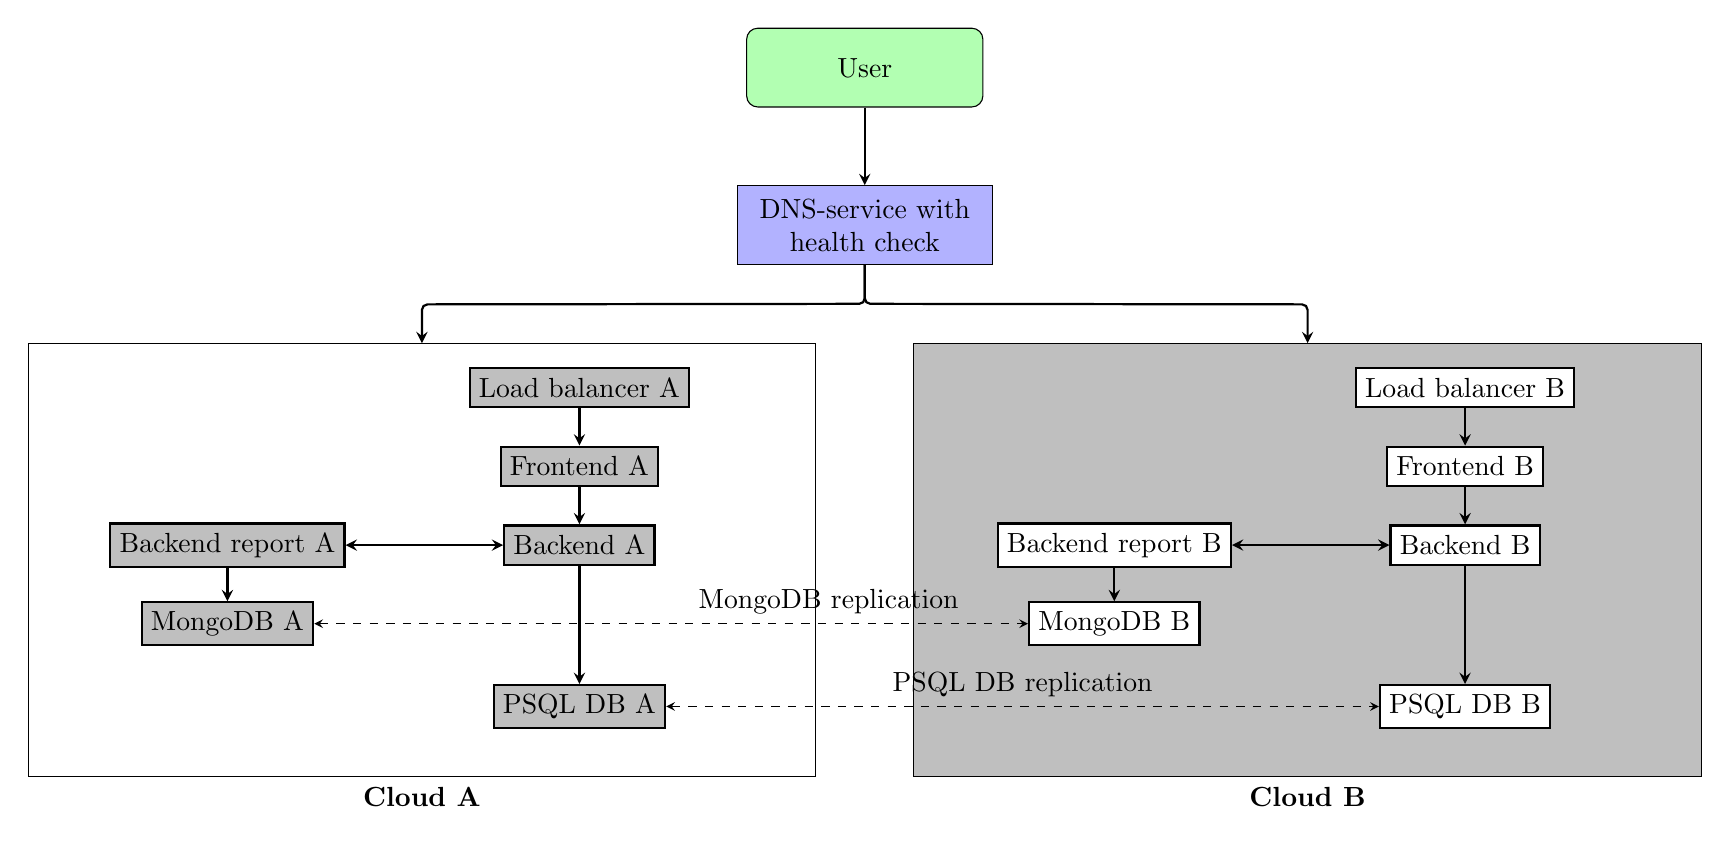
\begin{tikzpicture}[node distance=2cm]

% Draw user shape
\node (User) [user] {User};
% Draw DNS shape
\node (DNS) [dns, below of=User] {DNS-service 
with health check};


% Shapes for clouds 
\node (Cloud_A) [below=1.5cm of DNS.west, fill=none, draw=black, minimum width=10cm, minimum height=5.5cm, xshift=-4cm]{};
\node (Cloud_B) [below=1.5cm of DNS.east, draw=black, fill=gray!50,  minimum width=10cm, minimum height=5.5cm, xshift=4cm]{};
\node (Cloud_A_Label)[below=0cm of Cloud_A] {\textbf{Cloud A}};
\node (Cloud_B_Label)[below=0cm of Cloud_B]{\textbf{Cloud B}};
    
% Cloud A nodes
\node[block_A, below=3mm of Cloud_A.north, xshift=2cm] (Load_Balancer_A) {Load balancer A};
\node[block_A, below=1cm of Load_Balancer_A.north] (Frontend_A) {Frontend A};
\node[block_A, below=1cm of Frontend_A.north] (Backend_A) {Backend A};
\node[block_A, left=2cm of Backend_A] (Backend_Report_A) {Backend report A};
\node[block_A, below=1cm of Backend_Report_A.north] (MongoDB_A) {MongoDB A};
\node[block_A, below=1.5cm of Backend_A] (PSQL_DB_A) {PSQL DB A};

% Cloud B nodes
\node[block_B, below=3mm of Cloud_B.north, xshift=2cm] (Load_Balancer_B) {Load balancer B};
\node[block_B, below=1cm of Load_Balancer_B.north] (Frontend_B) {Frontend B};
\node[block_B, below=1cm of Frontend_B.north] (Backend_B) {Backend B};
\node[block_B, left=2cm of Backend_B] (Backend_Report_B) {Backend report B};
\node[block_B, below=1cm of Backend_Report_B.north] (MongoDB_B) {MongoDB B};
\node[block_B, below=1.5cm of Backend_B] (PSQL_DB_B) {PSQL DB B};

% Connection between user and DNS
\draw [arrow] (User) -- (DNS);

% Connection between DNS and clouds
\draw [arrow, rounded corners=2] (DNS.south) -- ($(DNS)+(0,-1)$) -- ($(Cloud_A)+(0,3.25)$) -- (Cloud_A.north);
\draw [arrow, rounded corners=2] (DNS.south) -- ($(DNS)+(0,-1)$) -- ($(Cloud_B)+(0,3.25)$) -- (Cloud_B.north);

% Connections inside cloud A
\draw [arrow] (Load_Balancer_A) -- (Frontend_A);
\draw [arrow] (Frontend_A) -- (Backend_A);
\draw [arrow_double] (Backend_A) -- (Backend_Report_A);
\draw [arrow] (Backend_Report_A) -- (MongoDB_A);
\draw [arrow] (Backend_A) -- (PSQL_DB_A);

% Connections inside cloud B
\draw [arrow] (Load_Balancer_B) -- (Frontend_B);
\draw [arrow] (Frontend_B) -- (Backend_B);
\draw [arrow_double] (Backend_B) -- (Backend_Report_B);
\draw [arrow] (Backend_Report_B) -- (MongoDB_B);
\draw [arrow] (Backend_B) -- (PSQL_DB_B);

% DBs replication
\draw [arrow_double_dashed] (MongoDB_A) -- node[anchor=south, xshift = 2cm] {MongoDB replication} (MongoDB_B);
\draw [arrow_double_dashed] (PSQL_DB_A) -- node[anchor=south] {PSQL DB replication} (PSQL_DB_B);
 

\end{tikzpicture}
\end{document}